
\section{Editor and REPL console}

Creation of user-friendly interface was an important part of the project.
The greatest challenge lied in finding the most intuitive way of presenting a complicated and highly advanced system. The main component was the language of regular expressions itself. User should be able to edit its code with ease. The second key feature was the ability to execute the code. 
In many Turing-complete languages, every expression can be evaluated into some value, which could the be printed back to the user. For example in python's REPL, typing $2+2$ yields $4$.
\begin{lstlisting}
>>> 2 + 2
4
\end{lstlisting}
and after running a regex, user obtains an object containing all matched groups
\begin{lstlisting}
>>> re.compile('a|b*').match('xxaxxbxxbbbx')
<re.Match object; span=(0, 0), match=''>
\end{lstlisting}
In Solomonoff the problem is not so trivial. The regular expressions could in principle be evaluated down to formal languages. For example 
\begin{lstlisting}
'a' ('b' | 'c' | 'ef' ) 'd'
\end{lstlisting}
would return a language consisting of strings
\begin{lstlisting}
'abd', 'acd', 'aefd'
\end{lstlisting}
The issue wish such approach is that not all languages are finite. The expression
\begin{lstlisting}
'a'*
\end{lstlisting}
would be evaluated as infinite set
\begin{lstlisting}
'', 'a', 'aa', 'aaa', ...
\end{lstlisting}
Some regexes, might be finite but of exponential size. For instance
\begin{lstlisting}
('0' | '1') ('0' | '1') ('0' | '1') ('0' | '1')
\end{lstlisting}
yields set of all bit-strings of length 4. Presenting user with the result in form of formal languages would be often impractical or impossible. 

As a result, our REPL does not evaluate expressions. The results of compilation are not printed in any form. Instead the interface is meant to be silent when compilation is successful. Only errors are printed. 

There are many different approaches to implement user interface for REPL.
One of them would be having a single editor window with all the code in it and the REPL output printed on the margins next to each respective line. This provides a very immersive user experience for Turing-complete languages. For regular expressions i'ts not as spectacular. Instead we decided to use two windows - one for code editor and the other for REPL console. All interaction with regular expressions is performed via special commands built into the console. Those commands could not be used inside the code editor, as they are not part of the language itself. In order to evaluate a transducer user would type the following line into REPL input
\begin{lstlisting}
:eval NAME 'input string'
\end{lstlisting}
Sometimes, user might want to see all the strings that belong to a given language. While there might be infinitely many of them, it's possible to ask user how large sample to generate. To achieve this the following line can be used
\begin{lstlisting}
:rand_sample NAME of_size NUMBER
\end{lstlisting}
Automata can also be interpreted as directed graphs. This property makes was used to further enhance user interface. Automaton's graph will be shown after typing this command
\begin{lstlisting}
:vis NAME
\end{lstlisting}
Those and many other functionalities have been implemented in the browser-based version of REPL. 

The implementation is not trivial. One of the ways to achieve such results would be by implementing a parser that could halt mid-parsing. For example user could first type
\begin{lstlisting}
x = ('x' |
\end{lstlisting}
and hit return button. The parser should notice that the expression is not finished and it has to wait for the next line of input.  Then as the user types the next line
\begin{lstlisting}
'y' )
\end{lstlisting}
a full and valid expression could be recognised and parser could return.
This approach is used by some programming languages. It's difficult to implement and requires the grammar to be appropriately structured. We later abandoned this idea due to the problematic nature of Solomonoff's grammar. In particular, it does not use semicolons to separate statements. For example
\begin{lstlisting}
x = 'a' 
y = 'b'
\end{lstlisting}
could be written in a single line
\begin{lstlisting}
x = 'a' y = 'b'
\end{lstlisting}
The equality sign determines start of new statement. By its very nature, parsing this, requires a lookahead of one token into the future. When the input is read in fragments, line by line, such a lookahead is not possible to obtain.
User could first type
\begin{lstlisting}
x = 'a' y
\end{lstlisting}
which would be recognized by parser as concatenation of string \texttt{'a'} with variable \texttt{y}. If the user then types
\begin{lstlisting}
 = 'b'
\end{lstlisting}
in the upcoming line, then the previous results of parsing would have to be discarded and the entire input reparsed again. Hence we decided to simplify the REPL and assume that every line of input fully defines the entirety of expression. As a result it's not possible to split input into multiple lines when using console. This is not a serious limitation, because multiline expressions could still be written in the editor window instead of console. 

The division of user interface into editor and console has one more advantage. It closely mimics the layout of command-line interface, where the typical workflow is to edit source code in local files using any text editor of user's choice and the REPL is kept open all the time alongside the editor. Many existing modes for Emacs follow similar convention.

The REPL is implemented on the server-side as a REST API endpoint. 
\begin{lstlisting}
@PostMapping("/repl")
public ReplResponse repl(HttpSession httpSession, 
    @RequestBody String line)
\end{lstlisting}
Every user has their own instance of REPL
\begin{lstlisting}
Repl repl = (Repl) httpSession.getAttribute("repl");
\end{lstlisting}
which holds a reference to the compiler and a set of built-in commands
\begin{lstlisting}
 public static class Repl {
    private static class CmdMeta<Result> {
        final ReplCommand<Result> cmd;
        final String help;
        final String template;
        
        private CmdMeta(ReplCommand<Result> cmd, 
               String help, String template) {
            this.cmd = cmd;
            this.help = help;
            this.template = template;
        }
    }
     
    HashMap<String, Repl.CmdMeta<String>> commands;
    OptimisedHashLexTransducer compiler;
}
\end{lstlisting}
whenever user types some command on the REPL console
\begin{lstlisting}
:cmd arg1 arg2 arg3
\end{lstlisting}
it gets parsed as
\begin{lstlisting}
String firstWord = "cmd";
String remaining = "arg1 arg2 arg3";
\end{lstlisting}
and then the appropriate command implementation is looked up in the map
\begin{lstlisting}
final Repl.CmdMeta<String> cmd = commands.get(firstWord);
return cmd.cmd.run(httpSession, compiler, log, debug, remaining);
\end{lstlisting}
The rest controller contains implementations of many such commands
\begin{lstlisting}
public static final ReplCommand<String> REPL_LIST = ...
public static final ReplCommand<String> REPL_EVAL = ...
public static final ReplCommand<String> REPL_RUN = ...
public static final ReplCommand<String> REPL_EXPORT = ..
public static final ReplCommand<String> REPL_IS_DETERMINISTIC = ...
public static final ReplCommand<String> REPL_LIST_PIPES = ...
public static final ReplCommand<String> REPL_EQUAL = ...
public static final ReplCommand<String> REPL_RAND_SAMPLE = ...
public static final ReplCommand<String> REPL_CLEAR = ...
public static final ReplCommand<String> REPL_UNSET = ...
public static final ReplCommand<String> REPL_RESET = ...
public static final ReplCommand<String> REPL_LOAD = ...
public static final ReplCommand<String> REPL_VIS = ...
\end{lstlisting}
All of those definitions above are lambda expressions that use library functions
of the compiler. The parameters taken by those lambda expressions are as follows
\begin{lstlisting}
public interface ReplCommand<Result> {
    Result run(
        HttpSession httpSession, 
        OptimisedHashLexTransducer compiler, 
        Consumer<String> log, 
        Consumer<String> debug, 
        String args) throws Exception;
}
\end{lstlisting}
As an example, consider the command 
\begin{lstlisting}
:eval f 'abc'
\end{lstlisting}
which evaluates transducer \texttt{f} for input string \texttt{'abc'}. 
On the frontend JavaScript will perform REST query
\begin{lstlisting}
const response = await fetch('repl', {
     method: 'POST',
     body: ":eval f 'abc'"
})
\end{lstlisting}
which will be received by server
\begin{lstlisting}
@PostMapping("/repl")
public ReplResponse repl(HttpSession httpSession, 
        @RequestBody String line) {
    Repl repl = (Repl) httpSession.getAttribute("repl");
    final String result = repl.run(
        httpSession, 
        line, // ":eval f 'abc'"
        s -> out.append(s).append('\n'), // console output
        s -> { } // debug logs are not displayed
    );
    ...
}
\end{lstlisting}
and the \texttt{repl.run} method will query the appropriate implementation to call for
the \texttt{:eval} command.
\begin{lstlisting}     
final String firstWord = "eval";
final String remaining = "f 'abc'";
final Repl.CmdMeta<String> cmd = commands.get(firstWord);
return cmd.cmd.run(httpSession, compiler, log, debug, remaining);
\end{lstlisting}
This in turn will trigger the following lambda function
\begin{lstlisting}
ReplCommand<String> REPL_EVAL = 
        (httpSession, compiler, logs, debug, args) -> {
    String[] parts = args.split("\\s+", 2); // f 'abc'
    String name = parts[0]; // f
    String input = parts[1]; // 'abc'
    G transducer = compiler.getTransducer(name);
    String output = compiler.specs.evaluate(transducer, input);
    return output == null ? "No match!" : output;
};
\end{lstlisting}
The output is sent back to JavaScript in form of JSON
\begin{lstlisting}
const replResult = JSON.parse(await response.text())
\end{lstlisting}
Remaining commands are implemented in a similar way.

Several of the functions may require access to HTTP session. In particular it's worth analysing the \texttt{:load} command. It's purpose is to emulate the process of loading source code from file. Whenever user types some code in the editor, it needs to be transported to server, then parsed and compiled. All the defined transducers results need to be saved for later use. The simplest way of achieving this, would be by extending the REST API as
\begin{lstlisting}
class ReplInput{
     String command;
     String editorContent;
}
public ReplResponse repl(
    HttpSession httpSession, 
    @RequestBody ReplInput)
\end{lstlisting}
and query it using
\begin{lstlisting}
const response = await fetch('repl', {
    method: 'POST',
    body: {
        command: replCommand,
        editorContent: editor.getValue()
    }
})
\end{lstlisting}
The downside of such solution is that the editor content could become large and sending it would require more internet bandwidth and time. Often user only wants to execute simple short REPL commands that do not require sending the entire code. Sometimes the code might be required but resending it might be omitted as long as user has not modified it. Hence the process of uploading code to the server has been delegated to a separate REST call.
\begin{lstlisting}
const response = await fetch('upload_code', {
     method: 'POST',
     body: code
})
\end{lstlisting}
The code is then stored in HTTP session, so the REST endpoint has a very simple implementation
\begin{lstlisting}
@PostMapping("/upload_code")
public void uploadCode(HttpSession httpSession, 
        @RequestBody String text) {
    httpSession.setAttribute("code", text);
}
\end{lstlisting}


Aside from the editor and REPL there is one more window on the webpage. It is dedicated for tutorial and short documentation.  While it does not enhance the functionality of the website per se, it plays an important role. The Solomonoff compiler is a very niche and specialised tool. There are no similar tools and any user coming to the website is not expected to be familiar with its usage. The primary purpose of the website is not to be a replacement for user's IDE and terminal. Instead it serves as an all-in-one introductory tutorial, interactive playground and a marketing campaign. We want to make the learning materials easily accessible and abundant. Building a strong community is the back-bone of every open-source project. 

\section{Design}

The website has seen numerous design changes. Since the beginning we knew there must be a way to interact with the code but the exact best way of presenting it to the user was not so self-evident. There exist numerous different approaches that are highly dependent on the language. For example the online  Java  compiler consists of only two windows - one for code and one for compiler output.
\begin{center}
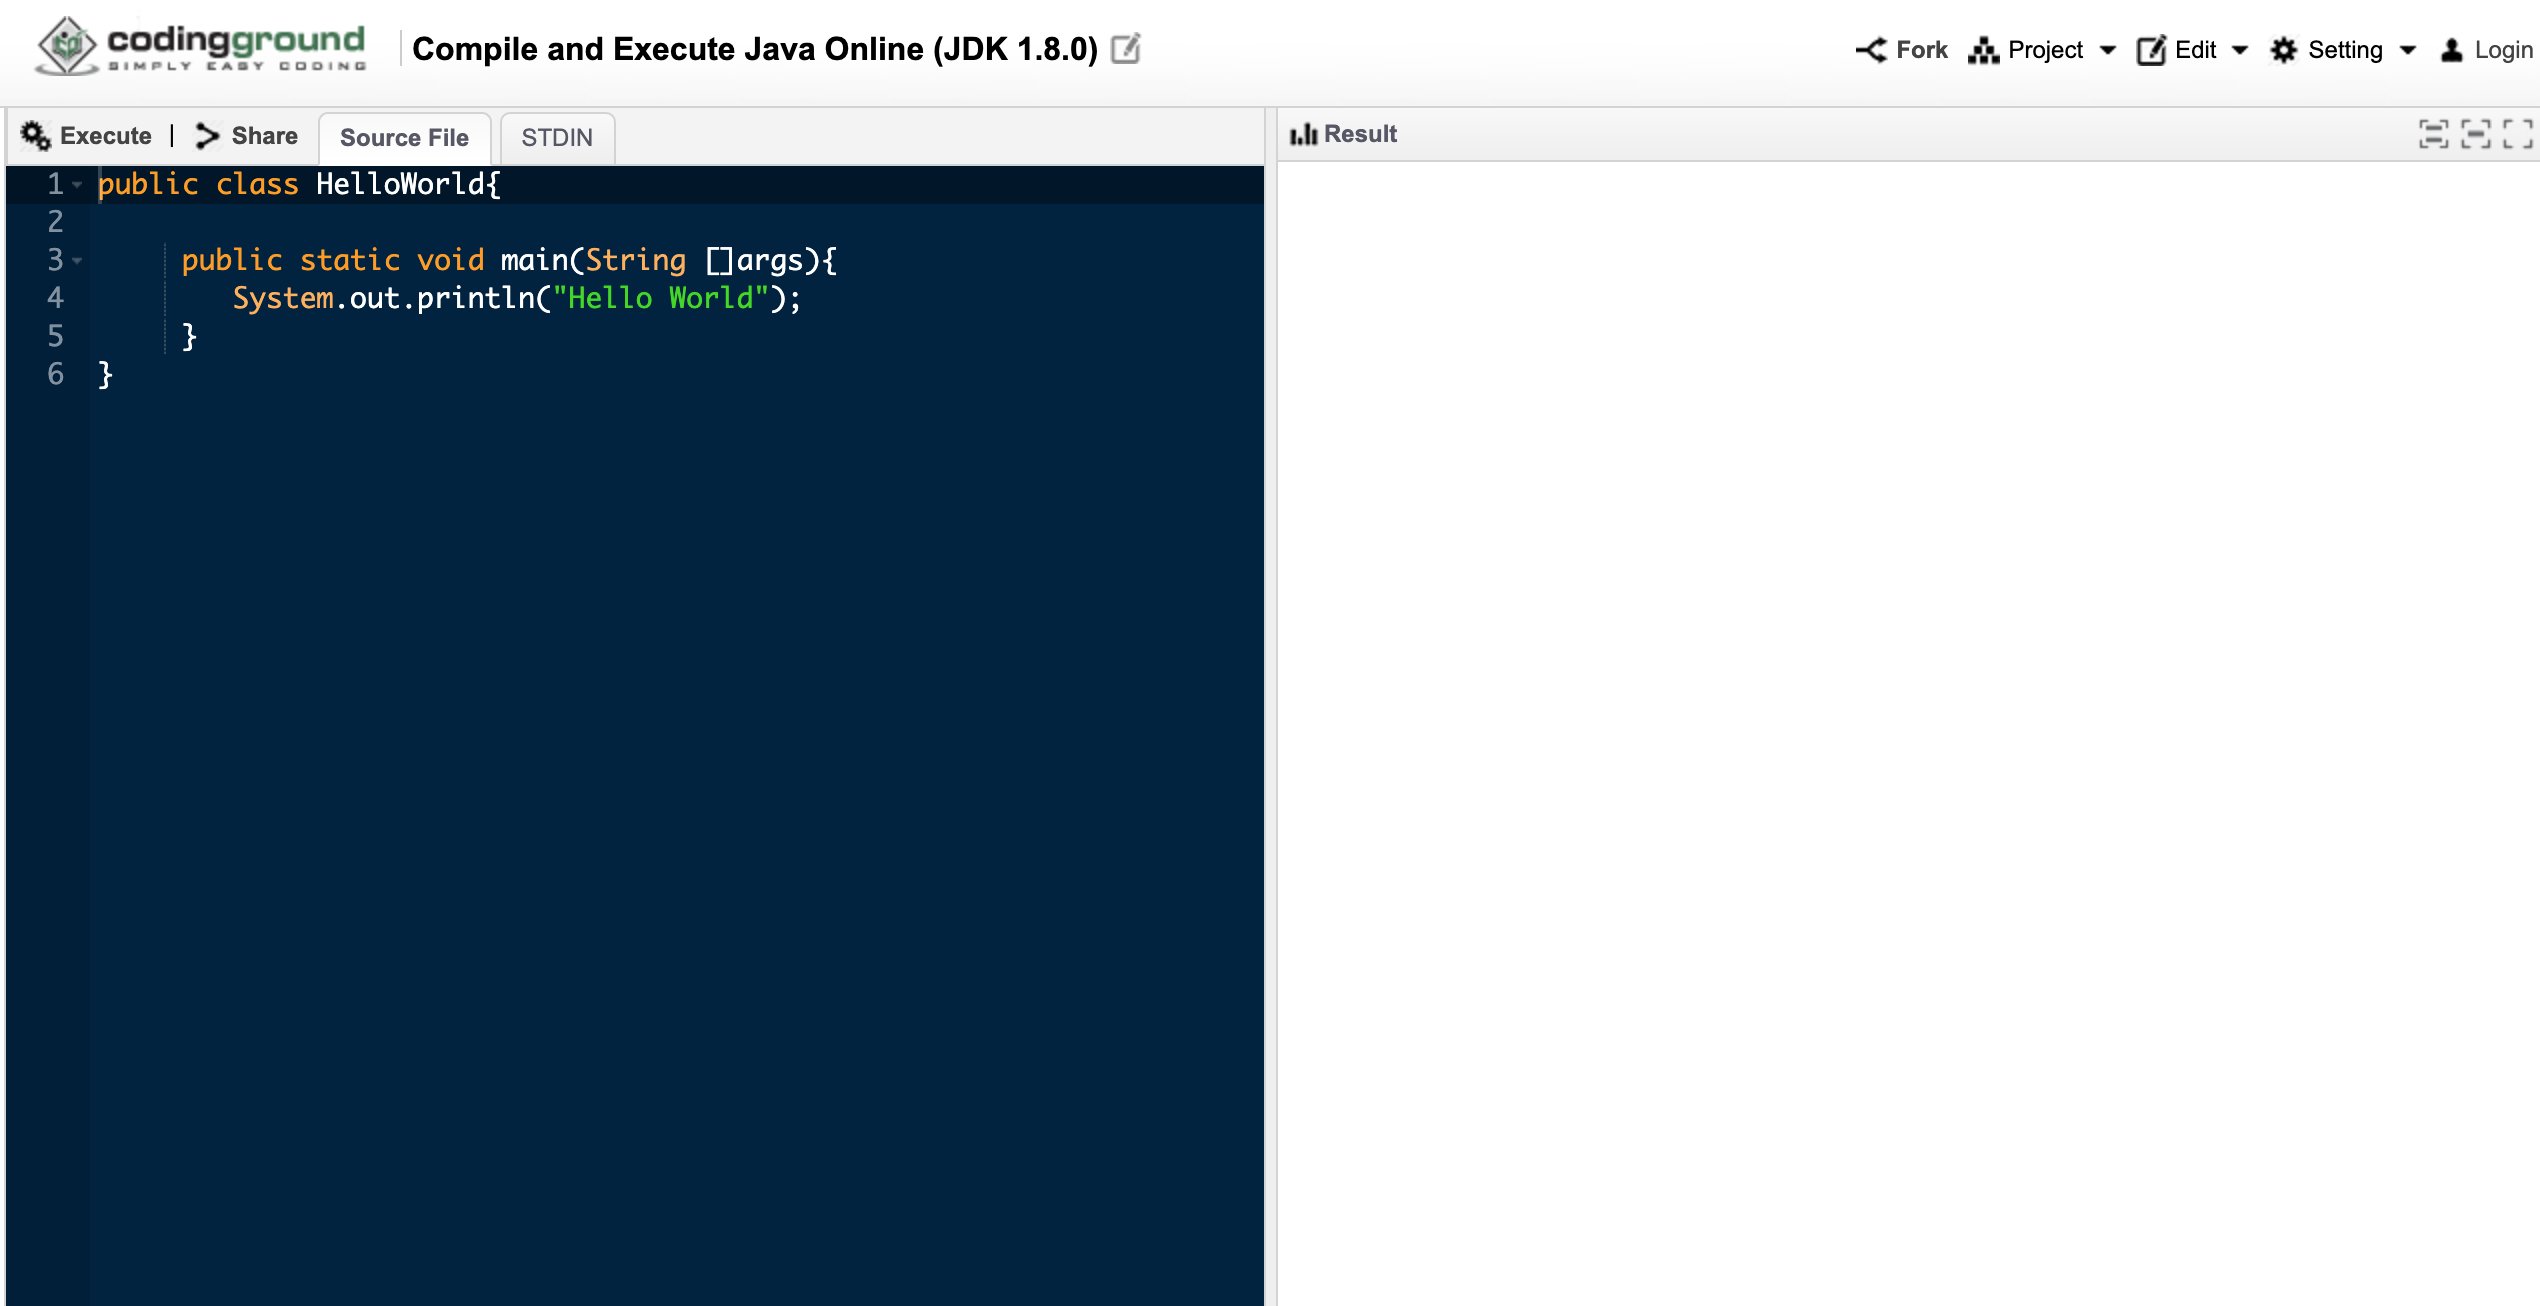
\includegraphics[scale=0.3]{java.png}
\end{center}
Java does not have REPL, hence there is no need to implement console input.
A slightly different has been taken by Haskell mode for emacs. 
\begin{center}
     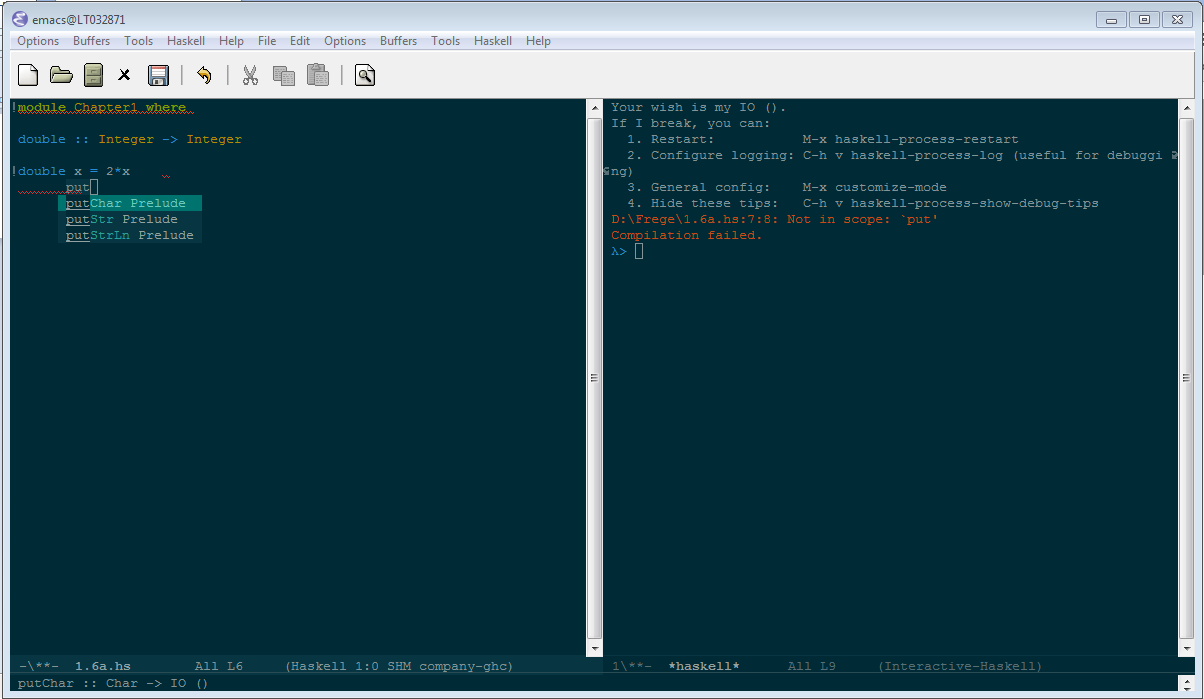
\includegraphics[scale=0.45]{haskell.png}
\end{center}
Here it is indeed possible to evaluate smaller snippets of code in the right window, while the left one is solely dedicated to editing local files that can be saved persistently. This is the approach that we settled for in our online playground for Solomonoff. 
\begin{center}
     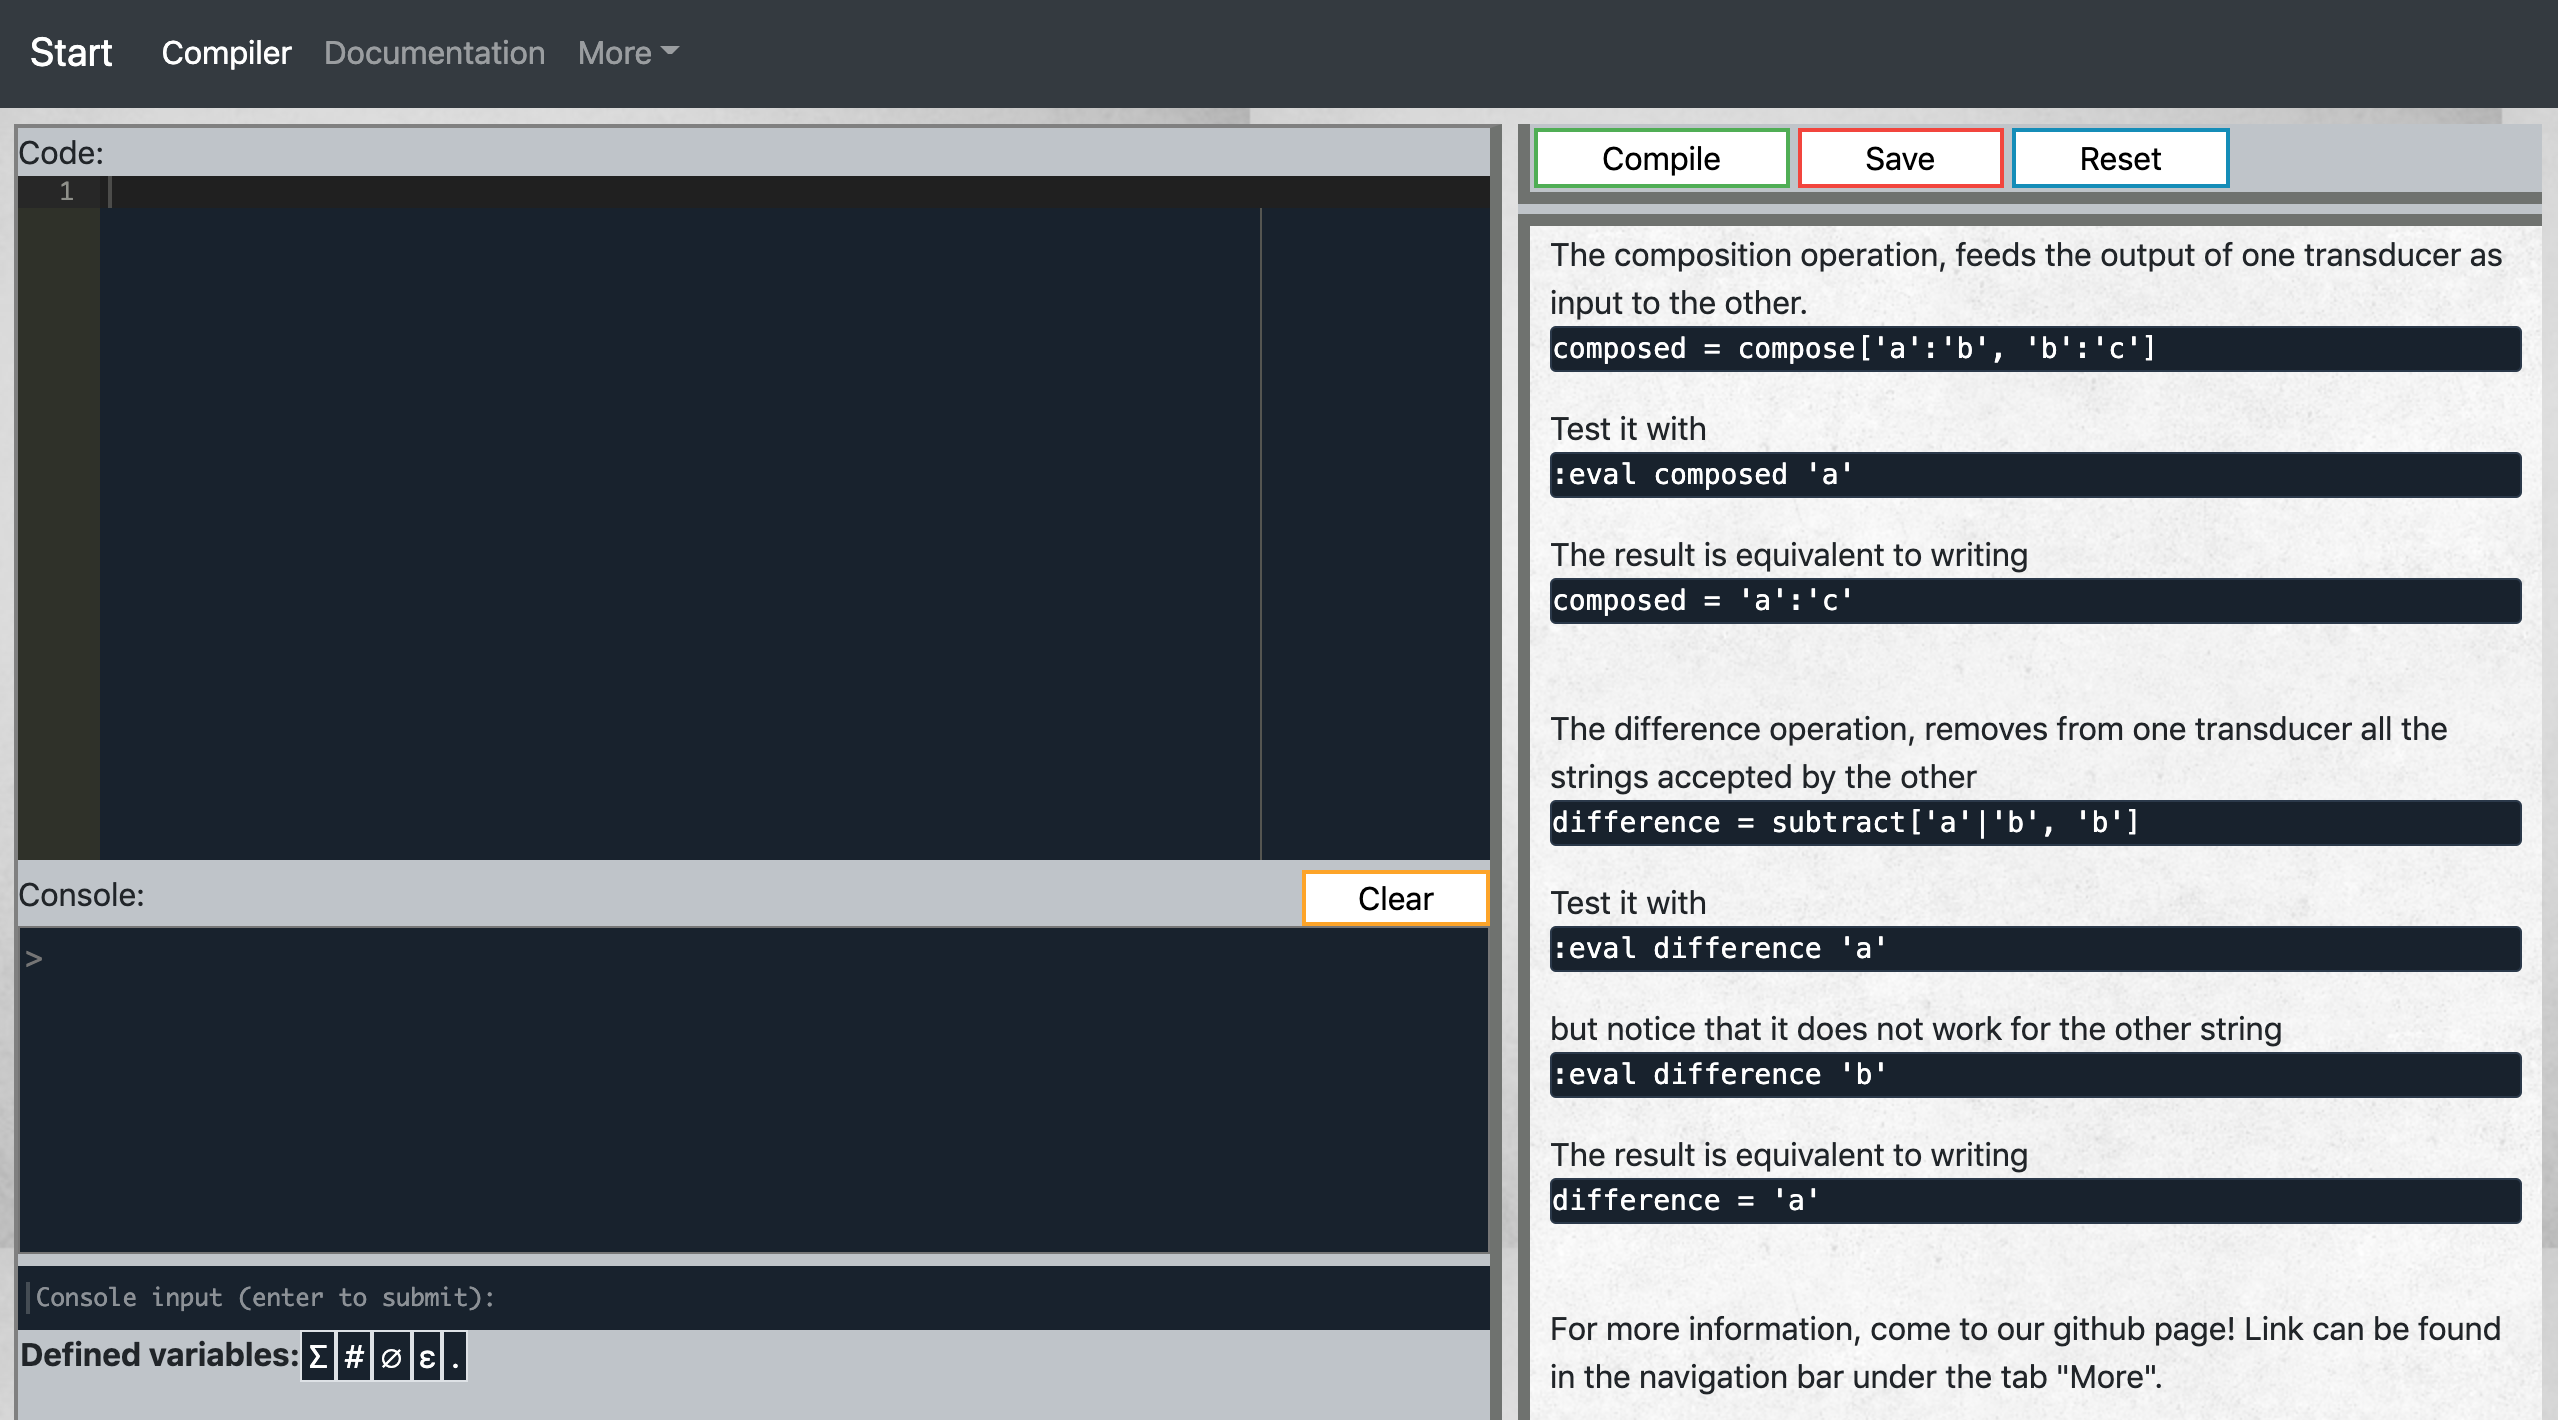
\includegraphics[scale=0.3]{web8.png}
\end{center}
Before reaching such final version we have experimented with another approach that seemed more natural for regular expressions. Here is an example of a similar website that evaluates UNIX regexes.
\begin{center}
     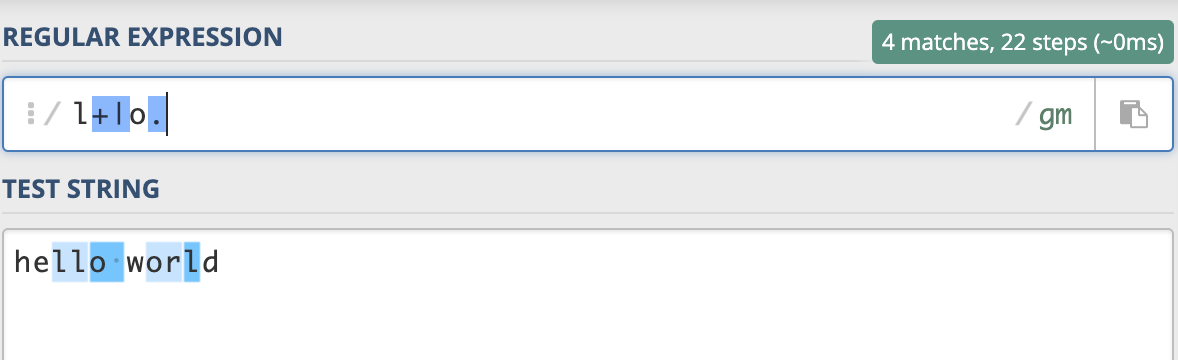
\includegraphics[scale=0.65]{regex.png}
\end{center}
Initially we tried to mimic such approach with some modifications. Solomonoff is much more complex than UNIX regexes. It allows variables, functions, comments and the overall code could consist of multiple lines. Hence a dedicated multiline editor window was required like in case of Java or Haskell.
\begin{center}
     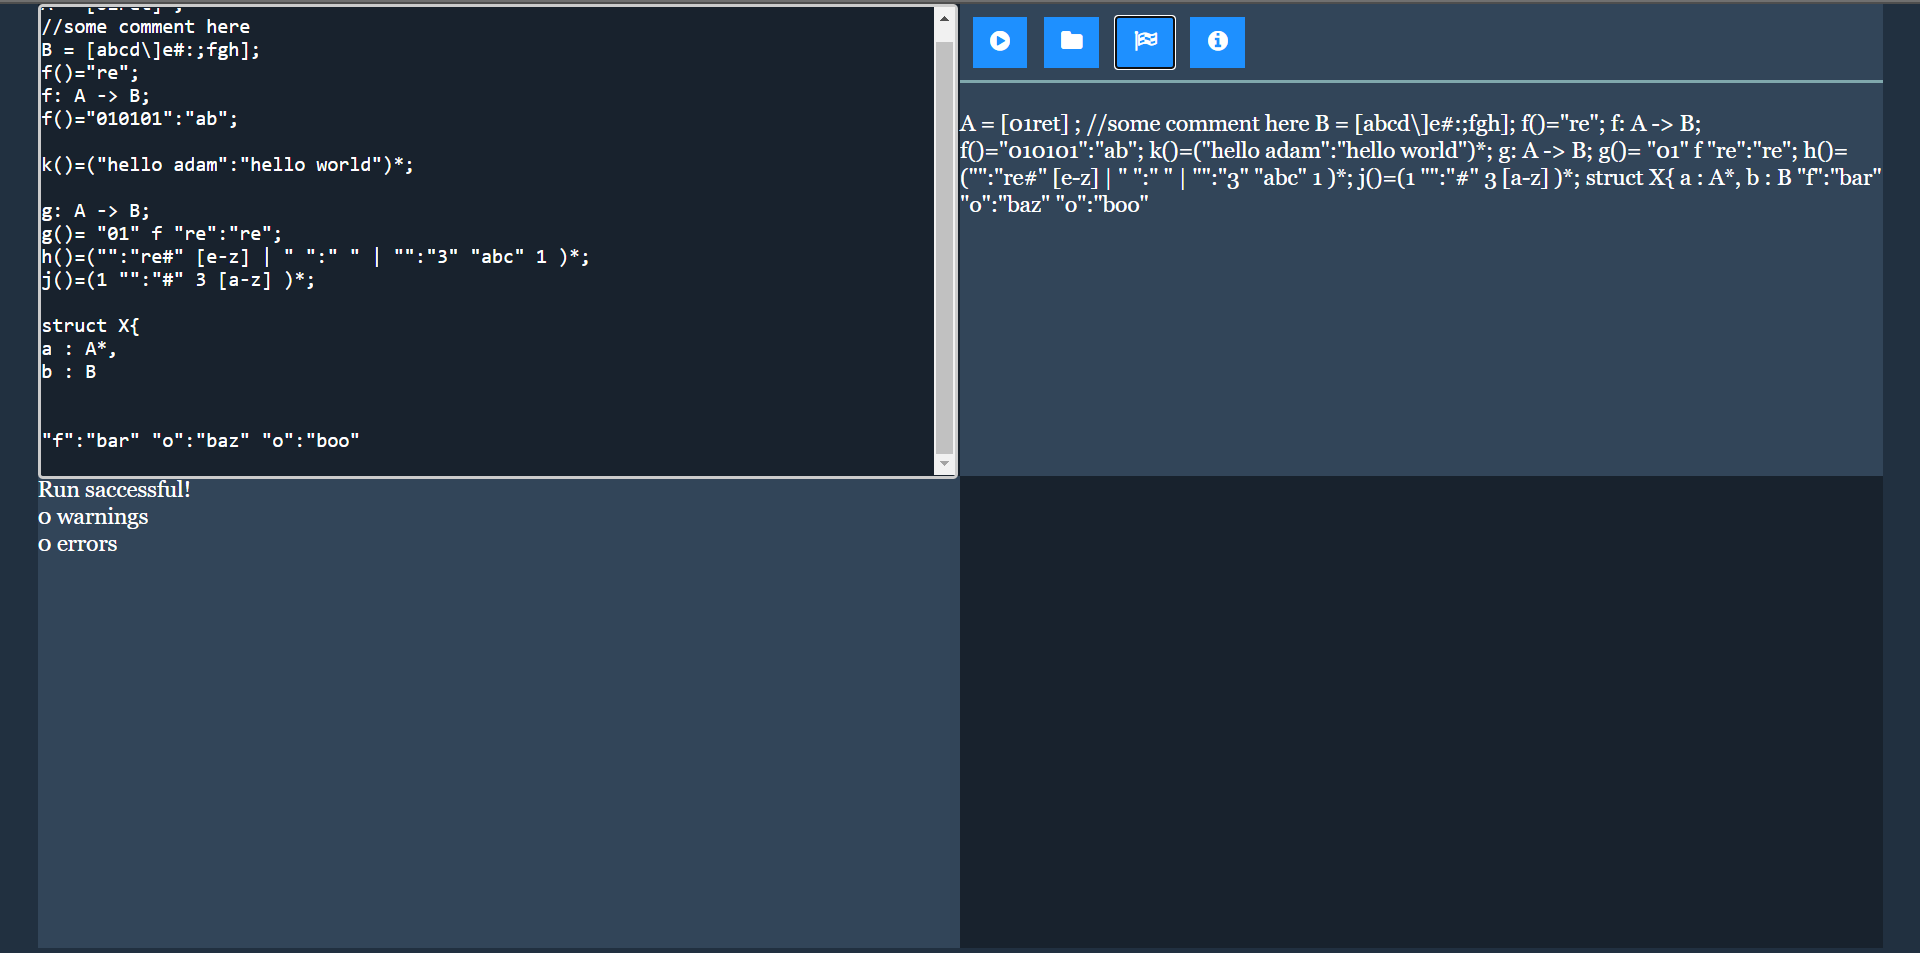
\includegraphics[scale=0.2]{web3.png}
\end{center}
The upper left window was dedicated to code. The lower left was meant to hold the test input string and the upper right would show the resulting transducer output. Such an approach seemed perfect at the beginning, when Solomonoff was still in early development. Over time, the language became increasingly complex. Several features were added that allowed for visualizing graphs of automata, sampling their languages, testing their formal properties and querying more complex information about them. The interface couldn't keep up with the full range of possibilities offered by he compiler. Hence, we decided to scrap the idea with two input-output windows and tried to emulate console-like REPL instead. The first version looked as follows
\begin{center}
     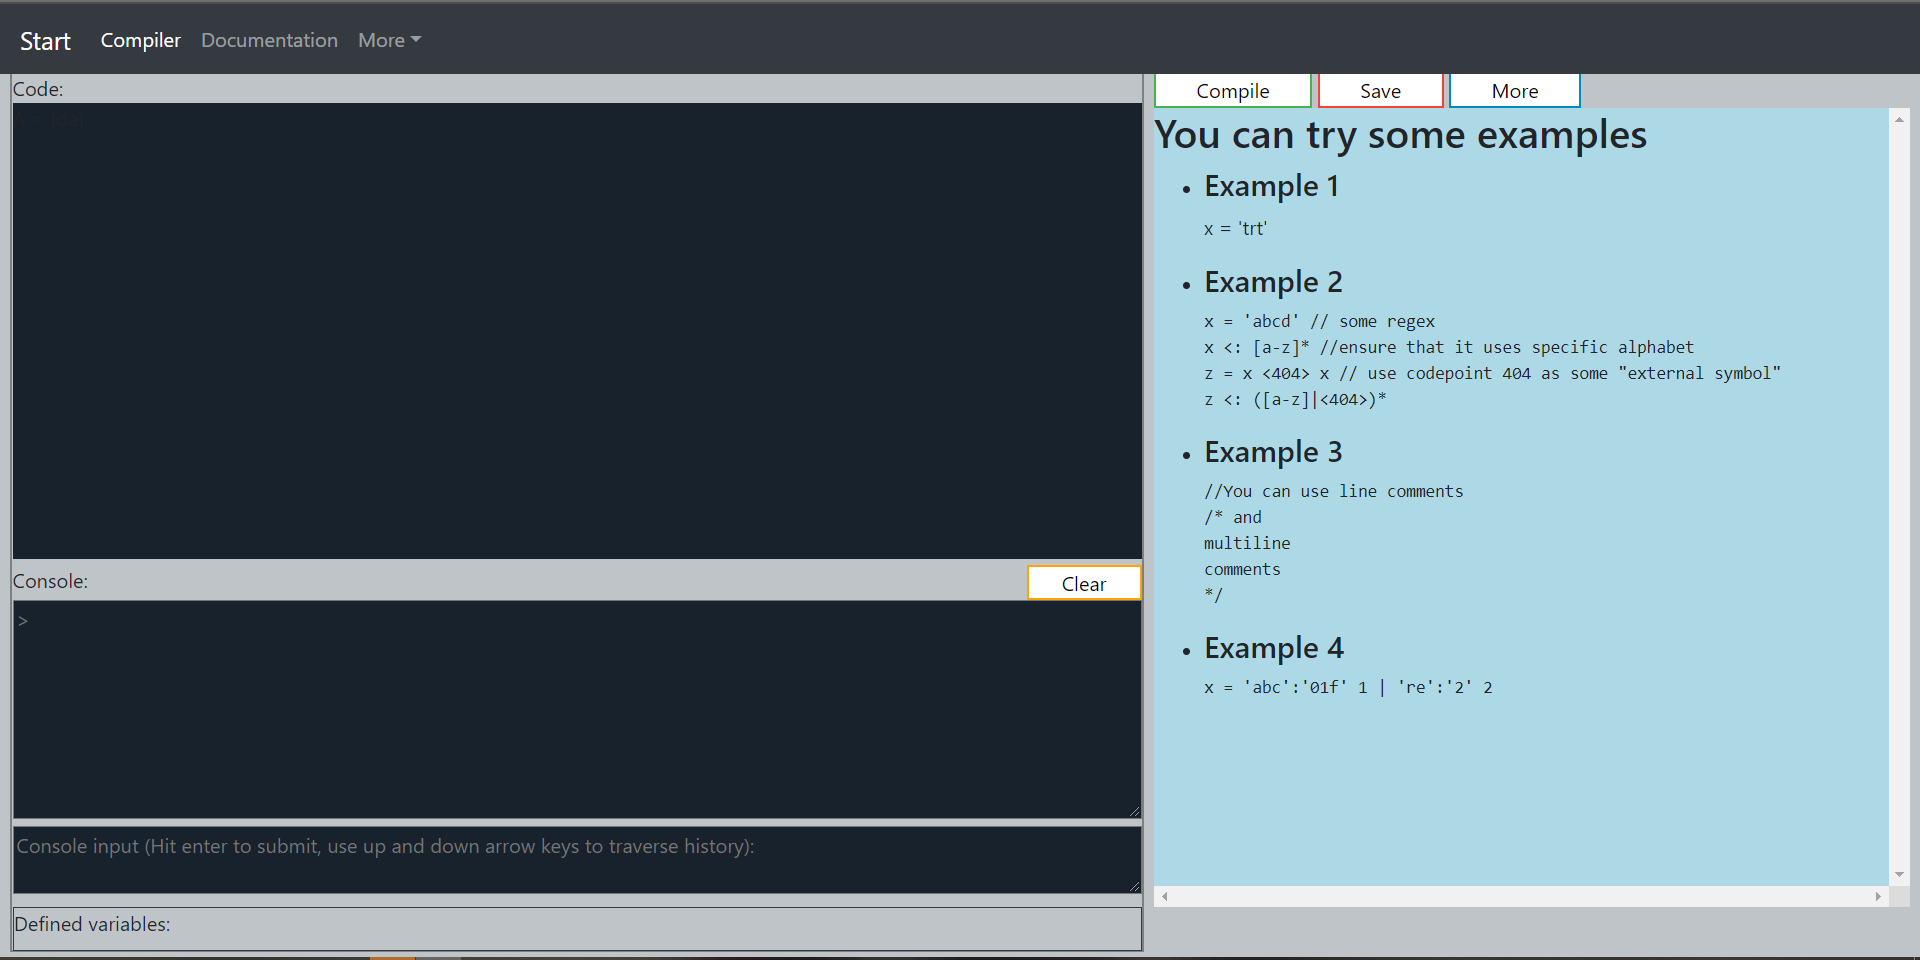
\includegraphics[scale=0.2]{web6.png}
\end{center}
It was at this point when we first tried to add a window for documentation. A great source of inspiration was the Alt-Ergo online playground. It comes with many helpful examples, which can be automatically copied to the editor upon clicking on them.
\begin{center}
     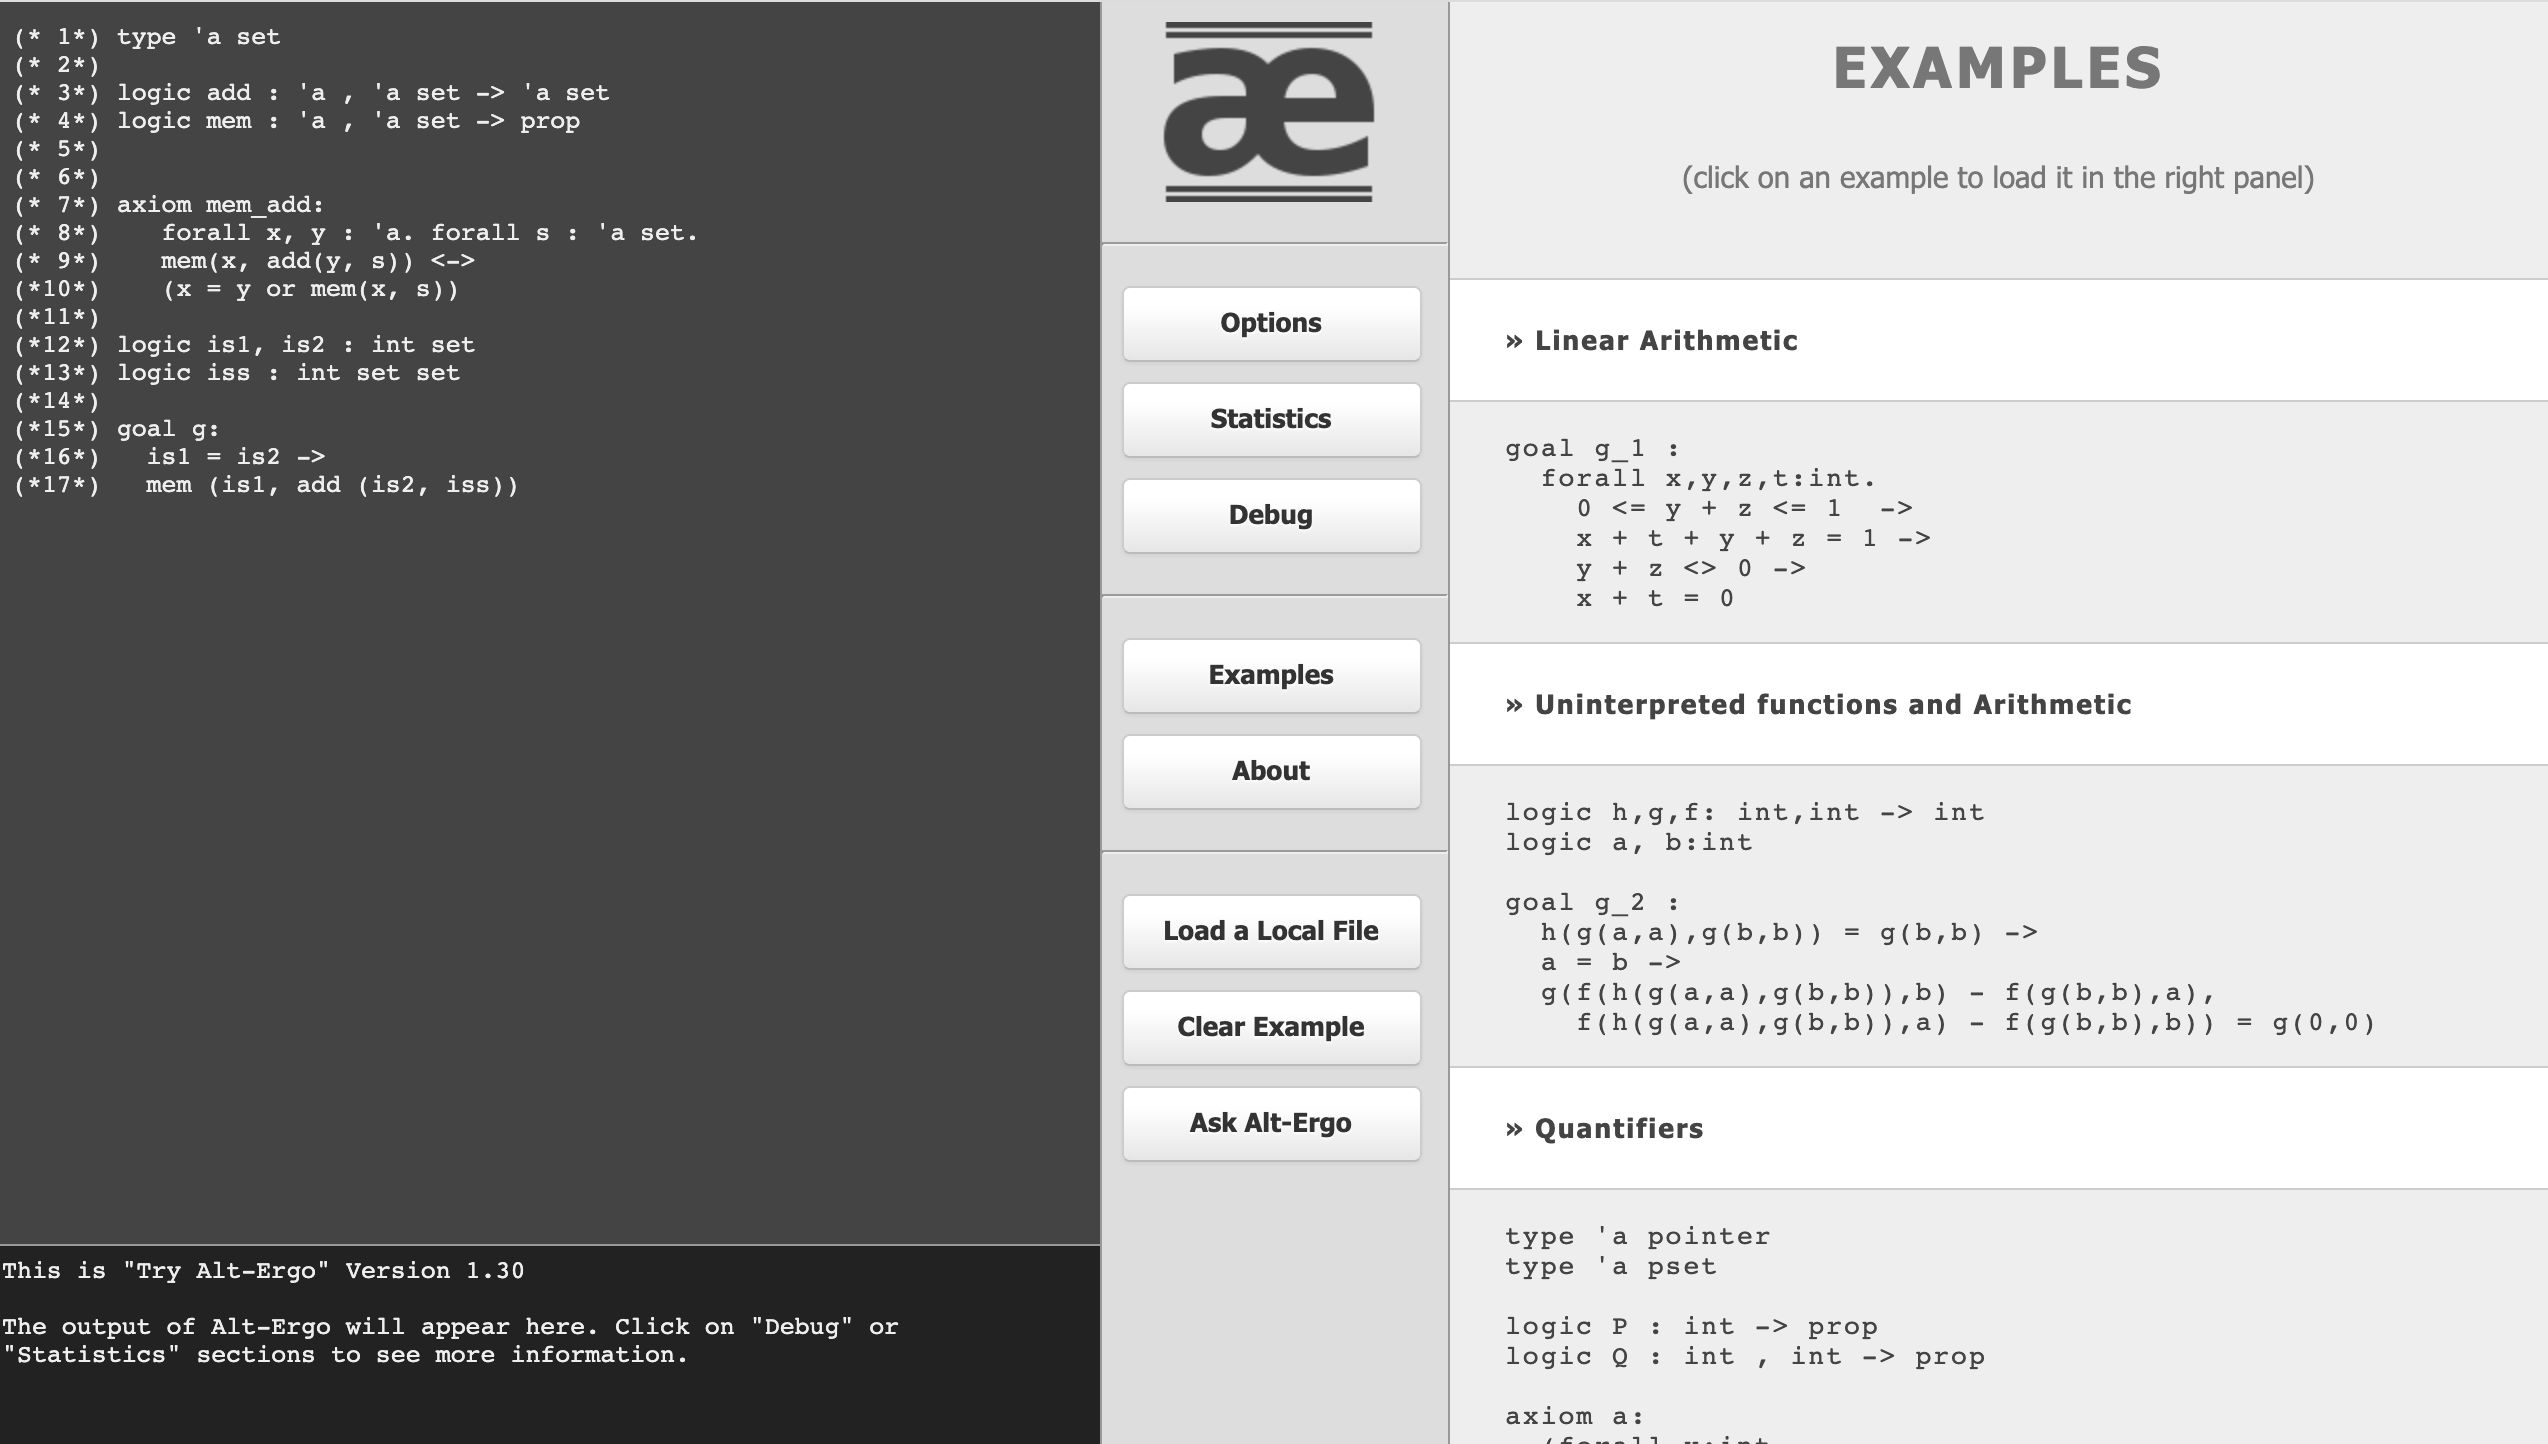
\includegraphics[scale=0.3]{alt-ergo.png}
\end{center}
Later we extended this idea to a full tutorial with explanations, rather than a simple list of copyable examples. 

\section{Ace editor}

At the same time as the layout of page evolved, we also actively developed the editor itself. While initially we used a simple HTML textarea element, we soon replaced it with the Ace editor. It allowed for integrating many additional features such as syntax highlighting, auto-suggestions, code snippets and marking errors. The core component of working with Ace was the necessity of developing our own syntax highlighting. All the previously mentioned come out-of-the box for existing languages, like JavaScript, C and Python. The matters get much more complicated, when one attempts to define their custom language. Ace documentation for syntax developers tends to be rather sparse. 

There exists a common framework followed by most syntax highlighters. Their configuration consists of two main components - the highlighting rules and the styling rules. The former consist of a set of regular expressions. Any region matched by a certain expression is marked with a list of styles. Then each style decides about the colour. Many existing text editors come with their own syntax highlighter and the required configurations may differ, albeit each format could be automatically converted into any other. 

By using the Iro editor, developer can develop only a single set of rules and then have them automatically converted to any other syntax highlighter. This includes support for Ace, SublimeText, TextMate and Atom. Most of the other editors, like Intellij, Eclipse, Notepad++ etc. use one of the above standards. 

The general format of Iro is as follows
\begin{lstlisting}

styles [] {
     
     .comment : style {
          color                 = #688557
          italic                = true
          ace_scope             = comment
          textmate_scope        = comment
          pygments_scope        = Comment
     }
 
}

main : context {
     
     : pattern {
          regex          \= (//.*)
          styles []       = .comment;
     }
 
}
\end{lstlisting}
each pattern matches some fragment of code and assigns a style to it. Then the style defines colour and scope. The scope is later used as a hint for various other tools that rely on syntax recognition. The colours themselves are also a mere hint. The end user might use an editor that supports various colour palettes. In particular many editors come with optional dark and light theme. Depending on user's choice, our colouring might be overriden. Hence the assigned scope is more important than the colour hint.

Most of the language grammars are context-free and cannot be recognized with a simple regular expression. Hence syntax highlighters allow for using stacks. A good example of this are the block comments. The regular expressions that apply outside of comments should not apply inside them. Iro allows developer to manipulate the stack using push and pop command.
\begin{lstlisting}
: inline_push {
     regex          \= (/\*)
     styles []       = .comment;
     default_style   = .comment
     : pop {
          regex       \= (\*/)
          styles []    = .comment;
     }
}
\end{lstlisting}
Solomonoff's syntax highlighter uses stack to correctly recognize comments and string literals enclosed in quotes and angle brackets. The rest of syntax highlighter is fairly simple and only matches key characters, such as equal signs, brackets, Kleene stars and union vertical pipes as well as variable identifiers.

After the syntax highlighter was developed, Iro automatically generated necessary Ace files. All those configurations are written JavaScript. In order to make them work, it's necessary to clone Ace's repository and compile the custom syntax along with the rest of sources. The compiled project needs to be hosted on website along with remaining JavaScript files. The Ace editor can be initialized using the following lines
\begin{lstlisting}
var editor = ace.edit("editor");
editor.session.setMode("ace/mode/mealy");
\end{lstlisting}
where \texttt{mealy} is the name of our custom syntax.
The editor has been styled using monokai theme
\begin{lstlisting}
editor.setTheme("ace/theme/monokai");
\end{lstlisting}
because its dark palette of colours gives the website a sharp and modern look. The dark theme is preferred by most users and is very popular nowadays. Moreover it's more relaxing to look at and doesn't irritate the eye. This point is especially important, because Solomonoff is targetted at tech-oriented audiences, so there is a good chance that our users will spend many hours looking at the editor. 

Solomonoff comes with several built-in functions. To make the interface more intuitive and ergonomic the editor needs to provide auto-suggestions with the full range available functions. Below is a list presenting some of the more important options.
\begin{lstlisting}
editor.setOptions({
     enableBasicAutocompletion: [{
          getCompletions: (editor, session, pos,
           prefix, callback) => {
               callback(null, [{
                    name: 'subtract[',
                    value: 'subtract[]',
                    score: 1,
                    meta: 'difference of two languages'
               },
               {
                    name: 'rpni!(',
                    value: 'rpni!()',
                    score: 1,
                    meta: 'RPNI inference algorithm'
               },
               {
                    name: 'rpni_mealy!(',
                    value: 'rpni_mealy!()',
                    score: 1,
                    meta: 'RPNI for Mealy machiens'
               },
               {
                    name: 'ostia!(',
                    value: 'ostia!()',
                    score: 1,
                    meta: 'OSTIA inference for transducers'
               },
               {
                    name: 'compose[',
                    value: 'compose[]',
                    score: 1,
                    meta: 'transducer composition'
               },
               {
                    name: 'inverse[',
                    value: 'inverse[]',
                    score: 1,
                    meta: 'transducer inversion'
               }
               ]);
          },
     }],
     enableSnippets: true,
     enableLiveAutocompletion: true
});
\end{lstlisting}
The \texttt{value} field is the text that autocompletion will produce when selected. The \texttt{meta} argument provides a short explanation that will be shown to the user. We decided to set \texttt{enableLiveAutocompletion} so that the dropdown box with all available functions will automatically show up as soon as the user starts typing. Some less experienced users might not be aware that the suggestions can be triggered manually by pressing \texttt{CTRL+SPACE}. The downside is that in some contexts the autosuggestion will pop up  despite not being necessary. This could irritate some users. Perhaps the best approach would be to make the auto-suggestions configurable. A user could set the editor properties according to their own liking. The only problem was that adding user customizations would increase the complexity of final product. Our goal was not to create a fully functioning IDE. The website is meant to work only as a showcase. Hence the final decision was to make the website as friendly to the newcomers as possible even at the cost of making the experienced users less comfortable. The general consensus was that users that like our product will quickly download the compiler locally and use it in conjunction with their own editor of choice. 

Initially, the Ace  was only used in the main editor window. The REPL console would be made of two text areas, one serving as editable input line and the other for console output, which was permanently set as non-editable. By design, the REPL commands could only be used in console and placing them in the main editor would only result in syntax errors. For instance
\begin{lstlisting}
:eval f 'input'
\end{lstlisting}
would only work in REPL, despite not being a valid Solomonoff code per se. As auto-suggestions were added, it became apparent that showing  REPL commands tin main editor would be very misleading
\begin{lstlisting}
editor.setOptions({
     enableBasicAutocompletion: [{
          getCompletions: (editor, session, pos,
          prefix, callback) => {
               callback(null, [
          ... 
               {
                    name: ':eval',
                    value: ':eval',
                    score: 1,
                    meta: 'evaluate transducer'
               }
          ...
               ]);
          },
     }],
     enableSnippets: true,
     enableLiveAutocompletion: true
});
\end{lstlisting}
On the other hand, not showing any hints related to REPL commands would seems like major shortcoming of the online playground. To address this issue it was later decided tha the REPL input line should also use Ace. As a result the website ended up with two instances of Ace editor. Both very similar to each other. The only difference being that auto-suggestions in REPL input would also display REPL commands, whereas the main code editor would not.

Using Ace in REPL input also happened to solve another problem. Every REPL command would have their own format of argument. For example the \texttt{:eval} would take transducer name and then some input string. The visualization only needs transducer name
\begin{lstlisting}
:vis f
\end{lstlisting}
 The most unintuitive is the random sample command which has two possible formats
 \begin{lstlisting}
:rand_sample f of_size 10
 \end{lstlisting}
and
 \begin{lstlisting}
:rand_sample f of_length 10
\end{lstlisting}
The former generates 10 random member strings, whereas the latter generates all member strings up to length of 10.
The \texttt{of\_size} and \texttt{of\_length} argument decides, which fo the two modes of generation to use. The initial idea to address this issue was to add user help displayed by the \texttt{:?} command.
\begin{lstlisting}
> :?
:vis [ID]
    Shows graph diagram of automaton
:rand_sample [ID] [of_size/of_length] [NUM]
    Generates random sample of input:output pairs produced 
    by ths transducer
:ls
    Lists all currently defined transducers
:clear
    Clears REPL console
:run [ID] [STRING]
    Runs pipeline for the given input
:unset [ID]
    Deletes a variable
:is_det [ID]
    Tests whether transducer is deterministic
:eval [ID] [STRING]
    Evaluates transducer on requested input
...
\end{lstlisting}
User could the consult this cheat sheet to determine format of arguments for each command. Such a solution was simple but it certainly didn't make for the most ergonomic user interface. With Ace it became possible to use code snippets instead.
Below are a few examples.
\begin{lstlisting}
getCompletions: (editor, session, pos, prefix, callback) => {
     callback(null, [
     {
          name: ':eval',
          value: ':eval',
          snippet: ':eval ${1:transducer_name} \'${2:input_string}\'',
          score: 1,
          meta: 'evaluate transducer'
     },
     {
          name: ':rand_sample of_size',
          value: ':rand_sample',
          snippet: ':rand_sample ${1:transducer_name} of_size ${2:number}',
          score: 1,
          meta: 'randomly generate sample'
     },
     {
          name: ':rand_sample of_length',
          value: ':rand_sample',
          snippet: ':rand_sample ${1:transducer_name} of_length ${2:number}',
          score: 1,
          meta: 'randomly generate sample'
     },
     ]);
}
\end{lstlisting}
The structure of arguments for each command was intuitively encoded in form
of blanks that need to be filled in each snippet. Each blank is specified using the \texttt{\$\{\}} braces.

